%% Comply with the comment where two consecutive percent symbols are written and then delete that comment.
%%
% Student Number: 2240357068
% Student Name: Baturay KAFKAS
% EEE @ Hacettepe University

% Last update: HH:MM DD/MM/YY

% My resource collection: https://github.com/kfksbtry/uni
% Circuits were set up in LTspice.

\documentclass{article}

\usepackage{comment}
\usepackage{graphicx}
\usepackage[top=25mm, bottom=25mm, left=25mm, right=25mm]{geometry}
\usepackage{amsmath}
\usepackage{moresize}
\usepackage{float}
\usepackage{fancyhdr}
\usepackage{booktabs}

\usepackage{pgfplots}
\pgfplotsset{width=10cm,compat=1.9}
\usepgfplotslibrary{external}
\tikzexternalize

\usepackage{lipsum} %% Delete this line later.

\pagestyle{fancy}
\fancyhf{}
\fancyhead[R]{Baturay KAFKAS 2240357068 Electrical \& Electronics Engineering}

\rfoot{\thepage}
\renewcommand{\headrulewidth}{0pt} 
\renewcommand{\footrulewidth}{0pt}



%%\setcounter{page}{[NUM]} Enter the next integer after the last page number used.



\begin{document}

\large %% Default font size

%%------------------------------------%%
{\textit{This part of the experiment is prepared with Online LaTeX Editor Overleaf, and the circuits are drawn in LTspice. Visit the website for the code here:}} %% May omit the circuit part or insert anything else in the preamble.

{\textbf{https://www.overleaf.com/read/[UPDATE HERE]}} %% Update the link.
\vspace{4mm}
\hrule
\vspace{4mm}
{\Large \textbf{[NUM]. PRELIMINARY WORK}} %% Enter the section number where the preliminary work is written in the document.

\vspace{4mm} %% Spacing
%%------------------------------------%%



%% Example question and its answer.
{\textbf{[NUM].1} \lipsum[1]} %% Edit the text.

\vspace{4mm} %% Spacing

{\textbf{Answer}: \lipsum[2]} %% Edit the text.



%% Example figure:

%%\begin{figure}[H]
%%    \centering
%%    \includegraphics[width=NUM\linewidth]{Draft1.png} Enter the width you'd like.
%%\end{figure}



%% Example table:

\begin{center}
    \large
    \begin{tabular}{ |c| c c| } 
    \hline
          & 1 & 2\\
        \hline
        a)& 3 & 4 \\
        \hline
        b)& 5 & 6 \\
        \hline
    \end{tabular}
\end{center} %% Rearrange the table.

%% Example graph

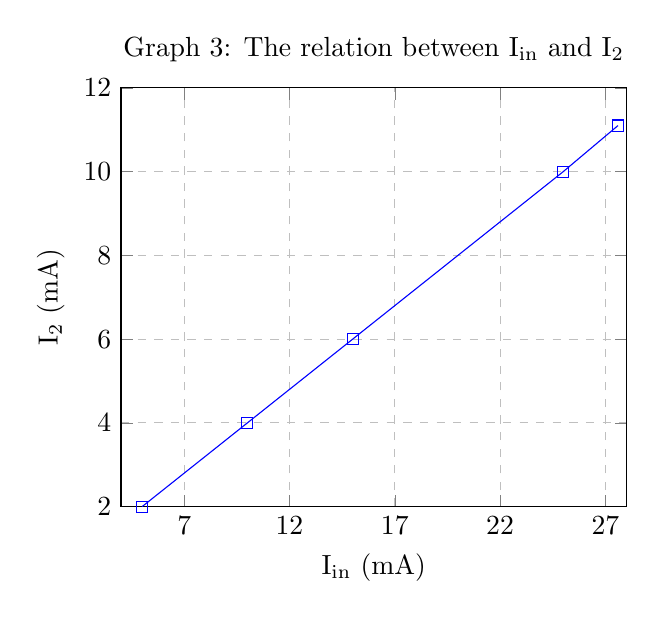
\begin{tikzpicture}
    \begin{axis}[
        title={Graph 3: The relation between I$_\text{in}$ and I$_\text{2}$},
        width = 8cm,
        xlabel={I$_\text{in}$ (mA)},
        ylabel={I$_\text{2}$ (mA)},
        xmin=4, xmax=28,
        ymin=2, ymax=12,
        xtick={2, 7, 12, 17, 22, 27},
        ytick={2, 4, 6, 8, 10, 12},
        legend pos=north west,
        ymajorgrids=true,
        xmajorgrids=true,
        grid style=dashed,
    ]
    
    \addplot[
        color=blue,
        mark=square,
        ]
        coordinates {
        (5,2)(10,4)(15,6)(25,10)(27.6, 11.1)
        };
    
    \end{axis}
\end{tikzpicture}

\end{document}